%!TEX root = ../../main.tex

\subsection{KarControl BDD}

\systemBDD{0.82}{KarControl}{KarControl}

\subsubsection{KarGruppe}
KarGruppe er den overordnede betegnelse for et vandkar med tilførende pH-værdi og gødningskoncentration. KarGruppen består af diverse sensorer og aktuatorer, og styrer et vilkårligt antal Sensor Ø’er. KarGruppen er styret af en controller, KarControl.

\subsubsection{Indløbsventil}
Indløbsventilen åbner og lukker for vandtilføjelsen til karret. Den bruges i forbindelse med, at der skal fyldes vand på karret. Det antages, at indløbsventilen er tilsluttet en vandforsyning, som altid er åben.

\subsubsection{Afløbsventil}
Afløbsventilen åbner og lukker for, at vand kan løbe ud af karret. Den bruges i forbindelse med, at karret skal tømmes.

\subsubsection{pH-Sensor}
pH-sensoren målet pH-værdien af gødningsblandingen i karret.

\subsubsection{Vandpumpe}
Vandpumpen pumper vand fra karret ud til Sensor Ø’erne.

\subsubsection{Flowmåler}
Flowmåleren måler mængden af vand, som tilføres karret gennem Indløbsventilen.


\subsection{KarControl IBD}

\systemIBD{0.82}{KarControl}{KarControl}

\subsubsection{RSIn}
RSConverter konverterer fra RS485 til RS232 når der modtages data fra CentralControl, og fra RS232 til RS485 når der afsendes data til CentralControl.

\subsubsection{RSOut}
RSConverter konverterer fra RS485 til RS232 når der modtages data fra KarControl, og fra RS232 til RS485 når der afsendes data til KarControl.

\subsection{Signal beskrivelser}

\begin{table}[H]
\centering
{\rowcolors{2}{white!80!black!30}{white!70!black!60} %farver på hver anden række -starter på 3
\setlength{\arrayrulewidth}{0.2mm}					 %tykkelse på linier 
\setlength{\tabcolsep}{10pt}						 %indryk i celle 
\renewcommand{\arraystretch}{1.5}					 %højden på tabelrum
\center
\begin{tabular}{|p{20mm}|p{40mm}|p{30mm}|p{30mm}|}		 %længden på alle rum
\hline

\multicolumn{4}{|>{\columncolor{white!20!black!90}}m{14.20cm}|}{\textcolor{white}{\large{\textbf{Signal beskrivelser}}}} \\\hline
\rowcolor{white!70!black!60}
\textcolor{black}{\large{\textbf{Navn}}}&
\textcolor{black}{\large{\textbf{Definition}}}&	
\textcolor{black}{\large{\textbf{Område}}}&
\textcolor{black}{\large{\textbf{Kommentar}}}\\
\hline
KarBus				& RS485 bus til kommunikation mellem enheder &	 	& Differentielt bussystem  \\
OeBus				& RS485 bus til kommunikation mellem enheder &	 	& Differentielt bussystem  \\
Data485				& RS485 bus til kommunikation mellem enheder &	 	& internt signal   \\
Data232				& RS485 konverteret til logisk niveau		 &	 	& Signal efter konvertering  \\
EnableIndløb		& Signal til at lukke vand ind i kar		 & 0-5V	& Signal til at styre magnetventil   \\
EnableAfløb			& Signal til at lukke vand ud af kar		 & 0-5V	& Signal til at styre magnetventil	\\
EnableVandpumpe		& Styre signal til pumpe			   	     & 0-5V & PWM styret signal	\\
Puls				& Takt tæller af flow				   	 	 & 0-5V & 	\\
pH					& Analog signal fra pH måler			 	 & fra -420 til 420 mV  & Analogt signal	\\
Indløb				& vandstyring i kar							 &    	& Til at lukke vand ind i kar	\\
Afløb				& vandstyring i kar	 						 &   	& Til at lukke vand ud af kar	\\
Dossering			& vandstyring til planter					 &      & Til at dosere vand til planterne	\\
\hline
\end{tabular}
}
\caption{signal beskrivelser for KarControl}
\label{table:SignalBeskrivelserKarControl}
\end{table}


%\subsection{KarControl Allokeringsdiagram}

%\begin{figure}[H]
%	\centering
%	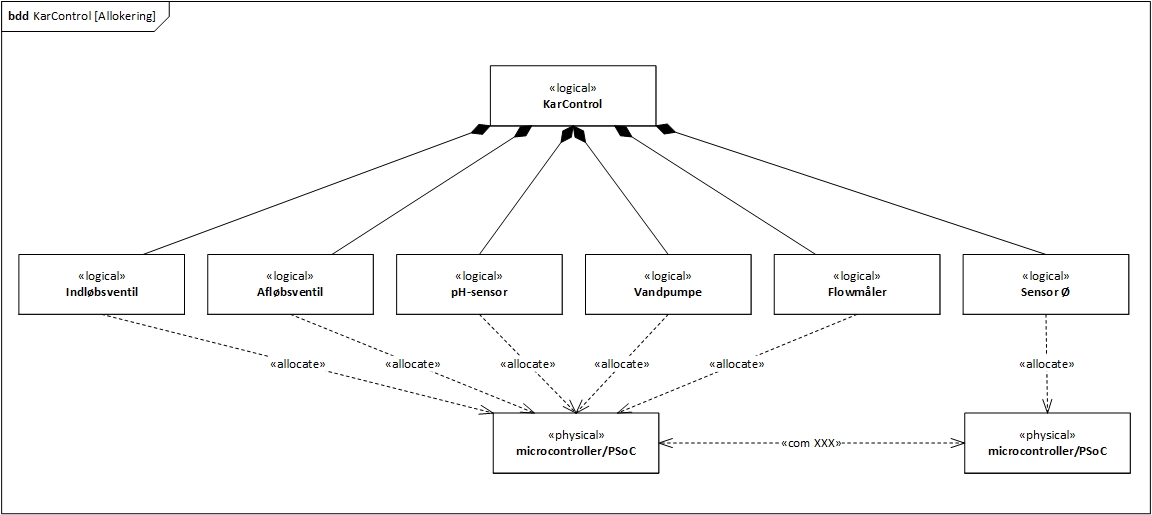
\includegraphics[width=0.82\textwidth]{Systemarkitektur/KarControl/KarControl_Allokeringsdiagram.png}
%	\label{fig:KarControl AD}
%	\caption{Allokeringsdiagram af KarControl}
%\end{figure}
